% TODO: Resumen
% TODO: 1, 2, 3, 4
% TODO: Refs y estilo de refs

\documentclass[12pt, a4paper]{article}
\usepackage[utf8]{inputenc}
\usepackage[spanish]{babel}
\usepackage[table]{xcolor}
\usepackage{url, hyperref}
\usepackage{graphicx, listings, xcolor, adjustbox, caption, subcaption, float}

\definecolor{codegreen}{rgb}{0,0.6,0}
\definecolor{codegray}{rgb}{0.5,0.5,0.5}
\definecolor{codepurple}{rgb}{0.58,0,0.82}
\definecolor{backcolour}{rgb}{0.95,0.95,0.92}

\lstdefinestyle{mystyle}{
    backgroundcolor=\color{backcolour},   
    commentstyle=\color{codegreen},
    keywordstyle=\color{magenta},
    numberstyle=\tiny\color{codegray},
    stringstyle=\color{codepurple},
    basicstyle=\ttfamily\footnotesize,
    breakatwhitespace=false,         
    breaklines=true,                 
    captionpos=b,                    
    keepspaces=true,                 
    numbers=left,                    
    numbersep=5pt,                  
    showspaces=false,                
    showstringspaces=false,
    showtabs=false,                  
    tabsize=2
}

\setlength{\parindent}{0pt}
\setlength{\parskip}{12pt}
\renewcommand{\arraystretch}{1.5}
\lstset{style=mystyle, language=Octave}

\title{\vspace{-3cm}Tarea 3: Función Rastrigin utilizando el algoritmo PSO}
\author{
    Universidad Autónoma de San Luis Potosí\\ 
    Facultad de Ingeniería - Ing. en Sistemas Inteligentes\\ 
    \textbf{Materia:} Cómputo Bioinspirado \\
    \textbf{Prof:} Dr. Cesar Augusto Puente Montejano  \\
    \textbf{Autor:} Angel de Jesús Maldonado Juárez
}
\date{\textbf{Fecha de entrega:} viernes 2 de septiembre de 2022}

\begin{document}

    \maketitle
    
    \begin{center}
        \rule{\textwidth}{0.5pt}
        \begin{abstract}
            \noindent Dentro del área de la inteligencia artificial, existe un enfoque que utiliza como fuente de inspiración a la naturaleza, en este reporte se habla de la \emph{Inteligencia de Enjambre}, el cual es un comportamiento presente en seres vivos que suelen estar en grupo. El algoritmo \emph{Particle Swarm Optimization} se basa en el movimiento que estos seres vivos tienen cuando están en conjunto, para poder generar población de \emph{partículas} y la posición de estas converjan a la solución de un problema. 
        \end{abstract}
        \rule{\textwidth}{0.5pt}
    \end{center}
    
    \section{Inteligencia de Enjambre}\label{title1}
        La \emph{Inteligencia de Enjambre} es un comportamiento presente en seres vivos que suelen actuar en grupo, la idea principal de este comportamiento es que existen individuos (\emph{agentes}) que forman parte de una población, y por si solos muestran una conducta bastante simple, pero cuando se observa a toda una población de individuos en conjunto, pareciera que hay coordinación y comunicación entre todos para lograr un común objetivo. Por ejemplo, una paloma por si sola vuela hacia cualquier dirección y en cualquier momento, pero cuando varias palomas vuelan en conjunto pareciera que alguien las estuviera guiando para ir hacia la misma dirección en el mismo momento. A este comportamiento presente específicamente en los pájaros se le conoce como \emph{bandada}.
    
    \section{Optimización por Enjambre de Partículas}
        Este algoritmo se basa en la \emph{Inteligencia de Enjambre} que se observa en la naturaleza, donde a cada individuo de la población del enjambre se le da un trato como \textbf{partícula}, generalmente se utiliza este enfoque para resolver \emph{problemas de optimización} (maximización  o minimización). Cada partícula en el enjambre tiene distintos \emph{componentes} que le ayuda a conseguir una comunicación con las demás partículas para trabajar en conjunto y lograr cumplir con el objetivo (resolver un problema). Estos componentes son:

        \begin{itemize}
            \item \textbf{Vector de posición} \((x, y)\)
            \item \textbf{Vector de velocidad} \((v_x, v_y)\)\
            \item \textbf{Inercia} (en base a su mejor posición \emph{local} y la mejor posición \emph{global})
        \end{itemize}

        Estos componentes son aplicados para representar el movimiento individual de las partículas en un enjambre. El \emph{espacio del problema} sería el lugar en el que pueden moverse las partículas, generalmente se representa con un plano en 2D o 3D. El \emph{vector de posición} representa la posición en la que se encuentra la partícula dentro del espacio del problema, el \emph{vector de velocidad} se utiliza para determinar hacia, y desde, donde se mueve la partícula y con cuanta rapidez. Finalmente, la \emph{inercia} actúa como una fuerza en el movimiento de la partícula que es influenciada por el estado en el que se encuentra la partícula (\emph{local}) y el estado del enjambre (\emph{global}).
        
        En la búsqueda de soluciones con este algoritmo, los componentes de las partículas deben actualizarse constantemente durante su ejecución, teniendo en cuenta que cada partícula debe tener conocimiento de sus propios movimientos y los del enjambre. Entonces, la posición de cada partícula puede ser representada como:

        \begin{equation}
            \vec{X_i^t}=[x_i^t,y_i^t]
        \end{equation}

        Donde, \(\vec{X_i^t}\) es el vector de la posición \(t\) de la partícula \(i\), representada por las coordenadas \(x_i^t\) y \(y_i^t\). Para representar el cambio de esta posición (movimiento) es necesario aplicarle cierta velocidad (distancia y dirección):

        \begin{equation}
            \vec{X_i^{t+1}}=\vec{X_i^t}+\vec{V_i^{t+1}}
        \end{equation}
        
        \(\vec{X_i^{t+1}}\) es la siguiente posición (\(t+1\)) de la partícula \(i\), representada por la posición actual \(\vec{X_i^t}\) de la partícula más el vector de velocidad \(\vec{V_i^{t+1}}\). Este último es el que crea la relación entre los componentes de una sola partícula con el enjambre, ya que, para calcularlo es de la siguiente forma:

        \begin{equation}
            \vec{V_i^{t+1}}=w\vec{V_i^t}+c_1r_1(\vec{P_i^t}-\vec{X_i^t})+c_2r_2(\vec{G^t}-\vec{X_i^t})\label{eq:3}
        \end{equation}

        Donde:

        \begin{itemize}
            \item \(w\vec{V_i^t}\): es el componente de inercia de la partícula, \(w\) representa los límites del problema, es decir, el rango de valores en los que se encuentra la posible solución.
            \item \((\vec{P_i^t}-\vec{X_i^t})\): representa el conocimiento que la partícula tiene sobre sus propios movimientos (\emph{componente cognitivo}), \(\vec{P_i^t}\) es la mejor posición de la partícula en la historia, \(\vec{X_i^t}\) es la posición actual de la partícula.
            \item \((\vec{G^t}-\vec{X_i^t})\): representa el conocimiento que la partícula tiene de su posición respecto al enjambre (\emph{componente social}), \(\vec{G^t}\) es la mejor posición que se ha encontrado en el enjambre en la historia, también puede interpretarse como la partícula con la mejor posición en el enjambre, \(\vec{X_i^t}\) es la posición actual de la partícula.
            \item \(c_1\) y \(c_2\): son \emph{constantes de atracción personal y global} respectivamente.
            \item \(r_1\) y \(r_2\): son números aleatorios entre \(0\) y \(1\), si estos no existieran el algoritmo puede quedarse en \emph{óptimos locales}.
        \end{itemize}

        Con la expresión (\ref{eq:3}) puede definirse un ciclo en el que la velocidad y la posición de cada partícula de un enjambre se actualice constantemente, de forma que al evaluar el \emph{fitness} (deseabilidad) de cada una se distinga la mejor partícula de todas y en base a ella, actualizar la posición y velocidad de todas las partículas del enjambre para la siguiente iteración del ciclo. De forma detallada, este algoritmo tiene los siguientes pasos:
    
        \begin{enumerate}
            \item Definición del problema: establecer una función/expresión que permita evaluar el \emph{fitness} de las partículas en cada iteración, también establecer los límites del problema, es decir, los rangos de valores que puede tomar la posición de una partícula.
            \item Definición de parámetros: dar un valor al \emph{coeficiente de inercia} \(w\) (máximo y mínimo), \emph{constante de atracción personal} \(c_1\), \emph{constante de atracción global} \(c_2\), \emph{tamaño de la población} \(n\), \emph{número de variables del problema} \(m\).
            \item Inicialización: se definen el número de iteraciones, la población inicial con posiciones, velocidades y mejor partícula inicial.
            \item Ciclo principal: actualizar velocidad y posición de las partículas, evaluar cada una y actualizar la mejor partícula global.
        \end{enumerate}
    
    \section{Función Rastrigin con el algoritmo PSO}
        La función \emph{Rosenbrock} es una función no convexa, que se utiliza como problema de prueba de rendimiento para algoritmos de optimización. Esta función está definida por:

        \begin{equation}
            f(x)=A_n+\sum_{i=1}^n[x_i^2-Acos(2\pi x_i)]
        \end{equation}

        Donde $A=10$ y $x_i\in [-5.12,5.12]$.
        
        En el proyecto de \emph{Octave} se define la función (problema) \lstinline{rastrigin(x)} en el archivo \lstinline{rastrigin.m}:
        
        \lstinputlisting{src/rastrigin.m}

        El algoritmo principal de PSO se define en el archivo \lstinline{run_PSO.m}, a continuación se muestra cada paso del algoritmo en código de \emph{Octave}:

        \textbf{Definición de los parámetros}
        \lstinputlisting{src/pso-parametros.m}

        \textbf{Inicialización}
        \lstinputlisting{src/pso-inicializacion.m}

        \textbf{Algoritmo principal PSO}
        \lstinputlisting{src/pso-algoritmo.m}

        La siguiente tabla muestra las distintas configuraciones de parámetros que se utilizaron para evaluar la función \emph{Rosenbrock} con el algoritmo PSO:

        \begin{table}[!ht]
            \begin{adjustbox}{width=\textwidth}
                \begin{tabular}{|c|c|c|c|c|c|c|c|c|}
                \rowcolor{yellow}
                \hline
                $LB$ & $UB$ & $n$ & $c_1$,$c_2$ & $w_1$,$w_2$ & $maxiter$ & Tiempo & $x_1,x_2,...x_{10}$ & $fitness$ \\
                \hline
                \([0,0,...]\) & \([5.9,5.9,...]\) & \(10\) & \(c_1=2,c_2=2\) & \(w_1=0.5,w_2=0.9\) & \(maxite=20\) & \(1.05309s\) & \(x_1=2.0410,x_5=2.9154,x_6=2.0306\) & \(18.683\) \\
                \hline
                \([0,0,...]\) & \([5,5,...]\) & \(10\) & \(c_1=2,c_2=2\) & \(w_1=0.5,w_2=0.9\) & \(maxite=20\) & \(1.04713s\) & \(x_n=0\) & \(0\) \\
                \hline
                \([0,0,...]\) & \([5,5,...]\) & \(9\) & \(c_1=2,c_2=2\) & \(w_1=0.6,w_2=0.9\) & \(maxite=19\) & \(0.907121s\) & \(x_n=0\) & \(0\) \\
                \hline
                \([0,0,...]\) & \([4.5,4.5,...]\) & \(9\) & \(c_1=1,c_2=2\) & \(w_1=0.719,w_2=0.9\) & \(maxite=19\) & \(0.893001s\) & \(x_n=0\) & \(0\) \\
                \hline
                \([0,0,...]\) & \([4,4,...]\) & \(8\) & \(c_1=1,c_2=1.2\) & \(w_1=0.85,w_2=0.99\) & \(maxite=18\) & \(0.768587s\) & \(x_n=0\) & \(0\) \\
                \hline
                \end{tabular}
            \end{adjustbox}
        \end{table}

        En base a esta tabla de resultados se puede observar que los parámetros que reduce o aumenta drásticamente el tiempo de ejecución son el \textbf{tamaño de la población (\lstinline{n})} y el \textbf{máximo número de iteraciones (\lstinline{maxiter})}, mientras más pequeños sean estos valores, más rápido arroja el resultado el algoritmo. Después están los \textbf{límites superior (\lstinline{UB}) e inferior (\lstinline{LB})}, estos límites indican el rango de valores que pueden tomar las variables del problema, y mientras más amplio sea este rango más grande será el \emph{espacio de búsqueda}, y por tanto aumenta la duración del algoritmo. Si se tiene un rango muy amplio en los límites, se puede aumentar el \textbf{número de partículas (\lstinline{n})} o el \textbf{número de iteraciones (\lstinline{maxiter})} para asegurarse de que hay las suficientes partículas para explorar el espacio, o que las partículas que ya hay tengan suficiente tiempo para explorar el espacio de búsqueda.

        \textbf{3 mejores resultados}:

        \begin{figure}[H]
             \centering
             \begin{subfigure}[b]{0.3\textwidth}
                 \centering
                 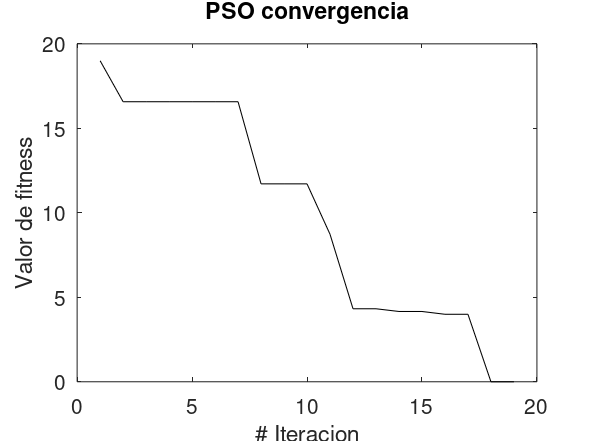
\includegraphics[width=\textwidth]{img/pso4.png}
                 \caption{Ejecución \#3}
                 \label{fig:pso4}
             \end{subfigure}
             \hfill
             \begin{subfigure}[b]{0.3\textwidth}
                 \centering
                 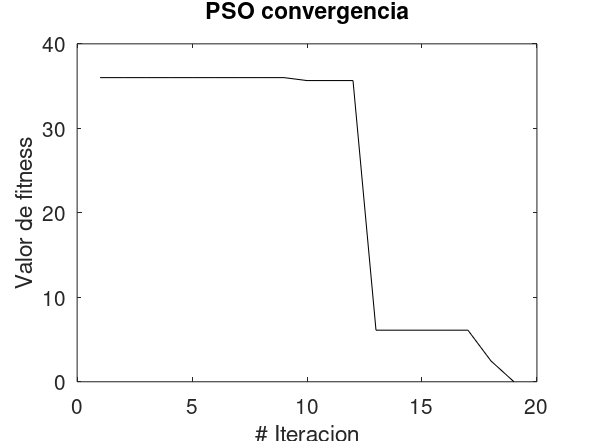
\includegraphics[width=\textwidth]{img/pso5.png}
                 \caption{Ejecución \#4}
                 \label{fig:pso5}
             \end{subfigure}
             \hfill
             \begin{subfigure}[b]{0.3\textwidth}
                 \centering
                 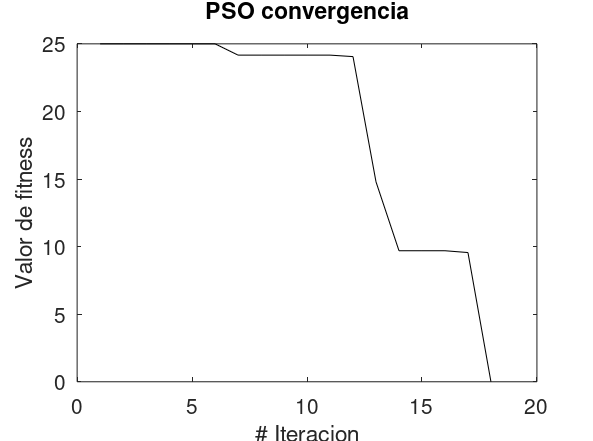
\includegraphics[width=\textwidth]{img/pso6.png}
                 \caption{Ejecución \#8}
                 \label{fig:pso6}
             \end{subfigure}
                \caption{Tres mejores ejecuciones del PSO con función Rastrigin.}
                \label{fig:psobest3}
        \end{figure}
        
    \section{Conclusiones}
        En base a los resultados mostrados en el experimento, se puede concluir que, mientras los límites del problema son más cercanos a la solución del problema, el número de partículas y el número de iteraciones es menor, el tiempo de ejecución del algoritmo disminuye drásticamente, sin embargo, la precisión disminuye, esto implica que deben de ajustarse \(c_1, c_2, w_1, w_2\) estos parámetros deben tener cierto \emph{balance} para conseguir una buena precisión en la solución del problema.

    \bibliographystyle{unsrt}
    \bibliography{refs}
    \nocite{*}
    
\end{document}
